\documentclass{article}

\usepackage{graphicx}
\usepackage{tikz}
\usepackage{tikzsymbols}
\usetikzlibrary{calc,patterns,shapes.geometric}
\pagestyle{empty}
\usepackage[margin=0pt]{geometry}
\geometry{papersize={14in,12in}}

\def\centerarc[#1](#2)(#3:#4:#5){\draw[#1] ($(#2)+({#5*cos(#3)},{#5*sin(#3)})$) arc (#3:#4:#5);}

\begin{document}
	\begin{figure}
		\centering
		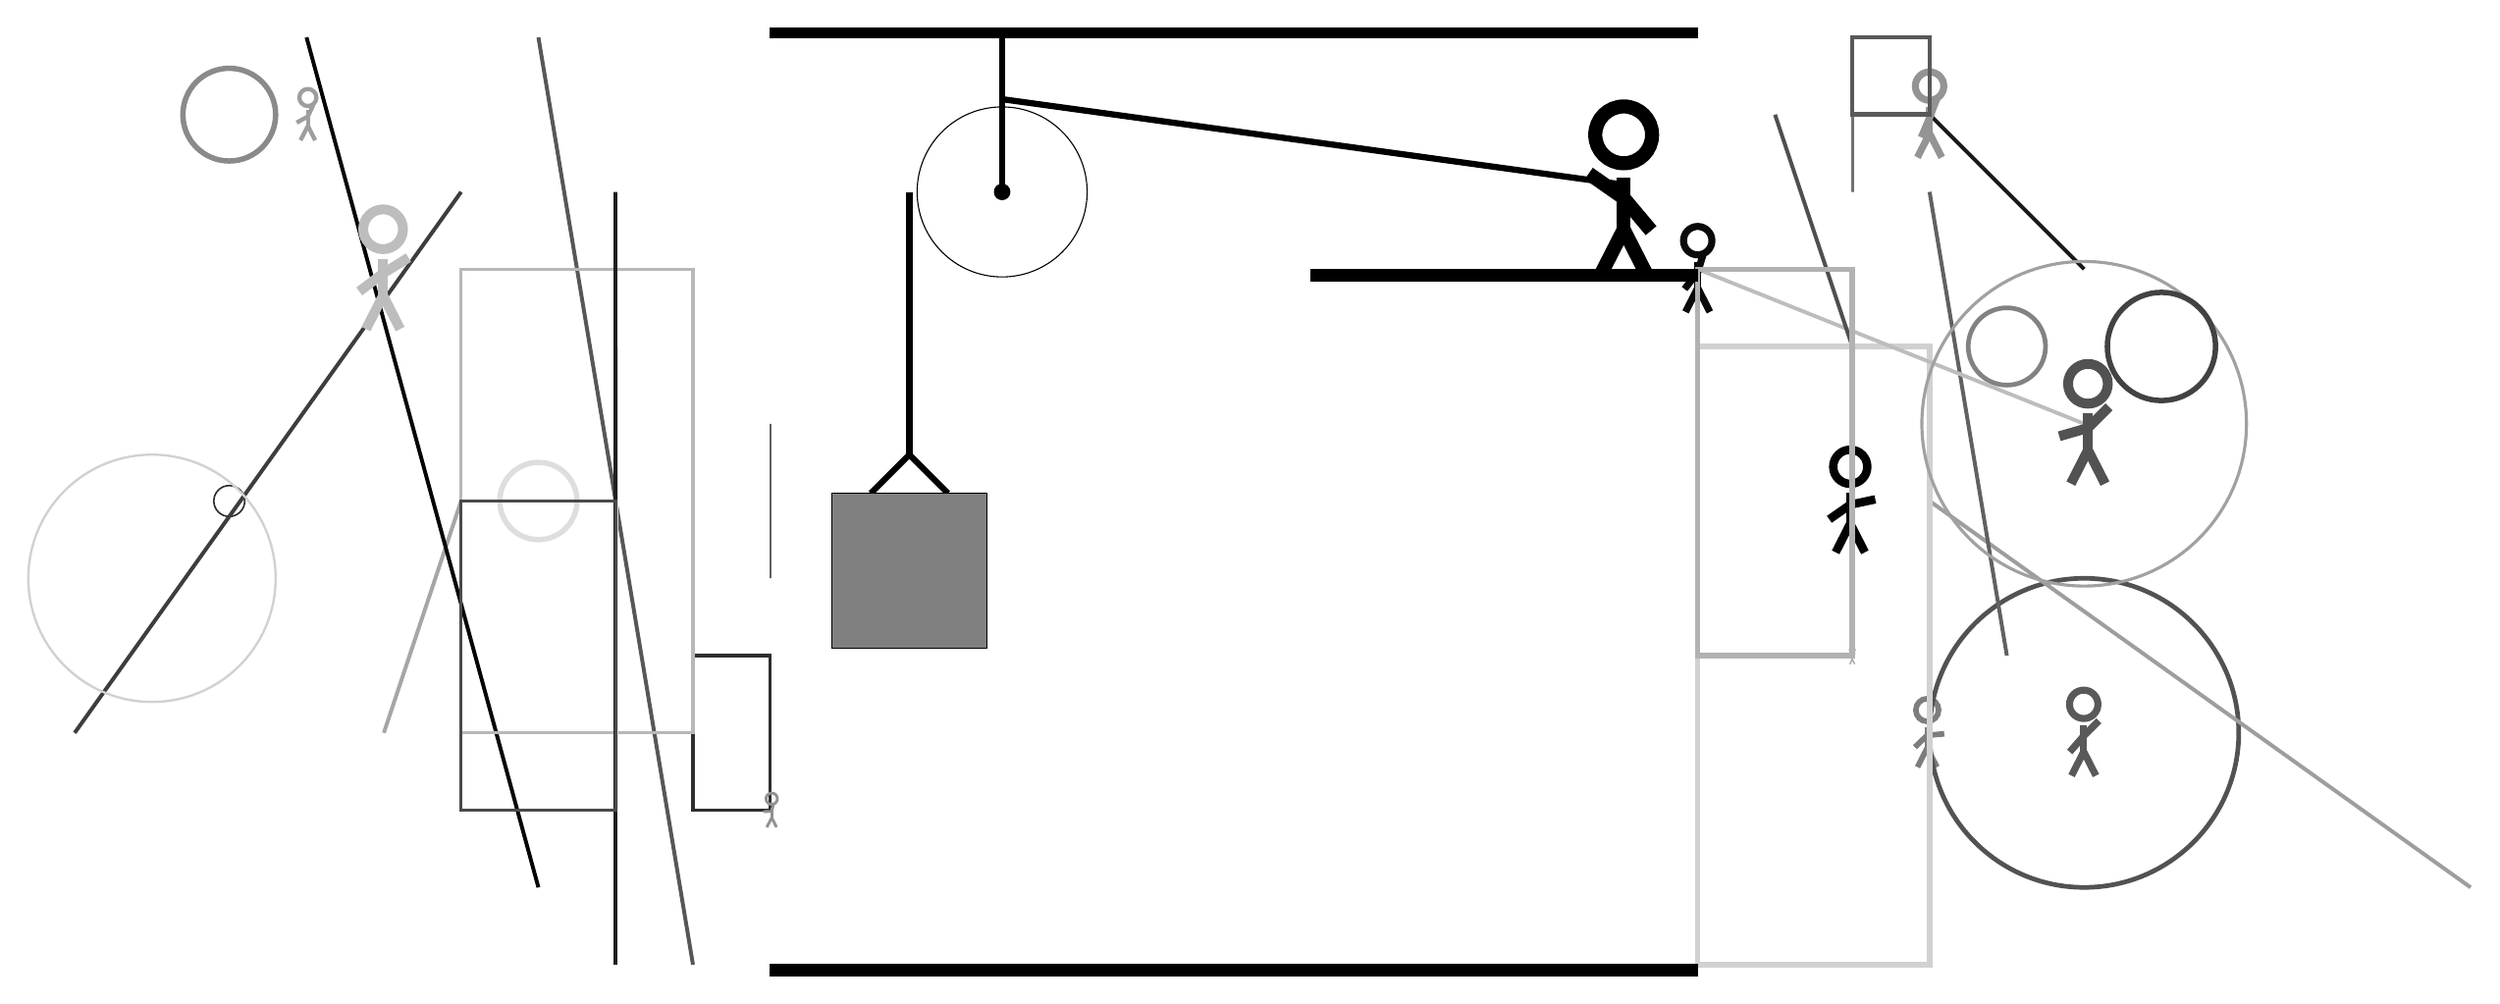
\begin{tikzpicture}
			%%%%% START %%%%%
			
			\draw[fill=black] (-2, 9) rectangle (10, 9.125);
			
			\draw (1, 7) circle (1.1);
			\draw[fill=black] (1, 7) circle (0.1);
			\draw[line width=0.8mm] (1, 9) -- (1, 7);
			
			\draw [line width=0.2mm, color=black!84](-9, 3) circle (0.2);
			
			\draw[line width=0.4mm, color=black!82] (-3, 1) rectangle (-2, -1);
			\node[line width=0.3mm, color=black!43] at (-2, -1) {\Strichmaxerl[2][2][76]};
			\node[line width=0.7mm, color=black!34] at (12, 1) {\Strichmaxerl[1][85][47]};
			\draw[line width=0.4mm, color=black!56] (12, 9) rectangle (12, 7);
			\node[line width=0.5mm, color=black!51] at (13, 0) {\Strichmaxerl[4][44][5]};
			
			\draw [line width=0.6mm, color=black!68](15, 0) circle (2.0);
			
			\draw[line width=0.5mm, color=black!38](13, 3) -- (20, -2);
			\draw[line width=0.5mm, color=black!90](15, 6) -- (13, 8);
			\draw[line width=0.5mm, color=black!66](-3, -3) -- (-5, 9);
			\draw[line width=0.5mm, color=black!76](-6, 7) -- (-11, 0);
			\node[line width=0.6mm, color=black!65] at (15, 0) {\Strichmaxerl[5][49][45]};
			\draw [line width=0.7mm, color=black!46](-9, 8) circle (0.6);
			\draw[line width=0.5mm, color=black!35](-6, 3) -- (-7, 0);
			\draw[line width=0.5mm, color=black!98](-5, -2) -- (-8, 9);
			\node[line width=0.5mm, color=black!42] at (13, 8) {\Strichmaxerl[5][67][69]};
			
			\node[line width=0.7mm, color=black!38] at (-8, 8) {\Strichmaxerl[3][29][65]};
			
			\draw[line width=0.7mm, color=black!18] (10, -3) rectangle (13, 5);
			\draw[line width=0.5mm, color=black!62](14, 1) -- (13, 7);
			\node[line width=0.2mm, color=black!26] at (-7, 6) {\Strichmaxerl[7][37][32]};
			\draw[line width=0.4mm, color=black!28] (-3, 0) rectangle (-6, 6);
			
			\draw [line width=0.6mm, color=black!49](14, 5) circle (0.5);
			
			\draw[line width=0.5mm, color=black!26](10, 6) -- (15, 4);
			\draw[line width=0.6mm, color=black!15] (-4, 5) rectangle (-4, -1);
			\node[line width=0.7mm, color=black!68] at (15, 4) {\Strichmaxerl[7][16][45]};
			
			\draw [line width=0.4mm, color=black!37](15, 4) circle (2.1);
			
			\draw [line width=0.3mm, color=black!18](-10, 2) circle (1.6);
			\draw[line width=0.5mm, color=black!88] (-4, -3) rectangle (-4, 7);
			\draw[line width=0.3mm, color=black!62] (-2, 4) rectangle (-2, 2);
			\draw[line width=0.6mm, color=black!65] (12, 9) rectangle (13, 8);
			\draw [line width=0.7mm, color=black!74](16, 5) circle (0.7);
			
			\node[line width=0.2mm, color=black!96] at (10, 6) {\Strichmaxerl[5][52][73]};
			\draw[line width=0.5mm, color=black!69](12, 5) -- (11, 8);
			\node[line width=0.2mm, color=black!99] at (12, 3) {\Strichmaxerl[6][35][12]};
			
			\draw [line width=0.7mm, color=black!13](-5, 3) circle (0.5);
			\draw[line width=0.7mm, color=black!30] (12, 1) rectangle (10, 6);
			
			\draw[line width=0.4mm, color=black!71] (-4, 3) rectangle (-6, -1);
			
			
			\draw[line width=0.8mm](-0.7, 3.1) --  (-0.2, 3.6) -- (0.3, 3.1);
			\draw[fill=black!50] (-1.2, 3.1) rectangle (0.8, 1.1);
			
			\draw[line width=0.8mm](-0.2, 7) -- (-0.2, 3.6);
			\centerarc[line width=0.8mm](1, 7)(90:180:1.2000000000000002)
			\draw[line width=0.8mm](1, 8.2) -- (9, 7.1);
			
			\node at (9, 7) {\Strichmaxerl[10][-35][-50]};
			\draw[fill=black] (5, 6) rectangle (10, 5.85);
			
			\draw[fill=black] (-2, -3) rectangle (10, -3.15);
			
			%%%%% END %%%%%
		\end{tikzpicture}
	\end{figure}	
\end{document}